\clearpage
\section{Operating procedures for Matrice 100 (J.~Lim)}
\label{app:OP}

\subsection{START OF DAY CHECKLIST}

\subsubsection{Firmware update}
\begin{enumerate}
\setlength{\itemsep}{0em}
\setlength{\parskip}{0em}
\item Ensure firmware is updated to the latest version
\end{enumerate}

\subsubsection{Battery charging}
\begin{enumerate}
\setlength{\itemsep}{0em}
\setlength{\parskip}{0em}
\item Ensure LiPo Battery are supervised at ALL times when charging
\item Look out for any puffing or inflating of battery in any state (charging or when stored)
\item Make sure tablet is fully charged and supervised when charging
\end{enumerate}

\subsubsection{Inventory Check}
\begin{enumerate}
\setlength{\itemsep}{0em}
\setlength{\parskip}{0em}
\item Make sure all all components of aircraft are in the aircraft case
\item Make sure extraction device is properly stored 
\end{enumerate}



\clearpage
\subsection{Go - No Go Checklist}
\textbf{Requirement to proceed: Must go through every item in above checklist}

\subsubsection{Weather}
Go: 
\begin{enumerate}
\setlength{\itemsep}{0em}
\setlength{\parskip}{0em}
\item Clear skies
\item Calm waters
\item Low precipitation
\item  Low wind speeds ($<\SI{22}{\meter\per\second}$)
\end{enumerate}

\textbf{No Go:}
\begin{enumerate}
\setlength{\itemsep}{0em}
\setlength{\parskip}{0em}
\item Any indication of rain, fog, thunderstorms
\item High wind speeds ($>\SI{22}{\meter\per\second}$)
\item Heavy waves
\end{enumerate}

\subsubsection{Equipment Status}
Go: 
\begin{enumerate}
\setlength{\itemsep}{0em}
\setlength{\parskip}{0em}
\item Frame- Check for no damage
\item Screw check- Ensure tightness (frame, standoffs, motors, camera)
\item Wire check- Ensure no damage (fraying, disconnections, etc)
\item Ensure gimbal is mounted correctly and tightly
\item Ensure extraction device is mounted correctly and tightly (when applicable)
\item Connection between tablet and aircraft are securely established
\end{enumerate}

\textbf{No Go:}
\begin{enumerate}
\setlength{\itemsep}{0em}
\setlength{\parskip}{0em}
\item Any damage found on frame 
\item Loose screws
\item Disconnected or exposed wires 
\item Gimbal not securely attached
\item Extraction device is loose and susceptible to hitting propellers
\item Unable to connect to aircraft through tablet
\item Lag or spotty response from remote controller or tablet
\end{enumerate}

\textbf{Requirement to proceed: Must go through every item in above checklist}







\clearpage
\subsection{DJI MATRICE 100 PREFLIGHT CHECKLIST}
\textbf{Note: GPS Mode assumed}

\subsubsection{Walk Around}
\begin{enumerate}
\setlength{\itemsep}{0em}
\setlength{\parskip}{0em}
\item Frame- Check for damage
\item Screw check- Ensure tightness (frame, standoffs, motors, camera)
\item Wire check- Ensure no damage (fraying, disconnections, etc)
\item Ensure gimbal is mounted correctly and tightly
\item Ensure extraction device is mounted correctly and tightly (when applicable)
\end{enumerate}

\subsubsection{Before Start}
\begin{enumerate}
\setlength{\itemsep}{0em}
\setlength{\parskip}{0em}
\item Verify all batteries are full
\begin{enumerate}
\setlength{\itemsep}{0em}
\setlength{\parskip}{0em}
\item Verified by pressing power button once
\item Full battery status if, all four bars are lit 
\item If all lights are lit, charge battery if possible
\end{enumerate}
\item Select battery and attach (\textbf{Do NOT connect to JST})
\item Attach propellers. \textbf{Ensure correct rotation}, screw check
\begin{figure}[h]
\begin{center}
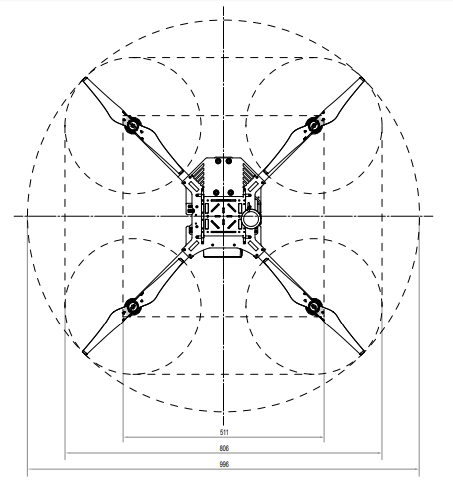
\includegraphics[width=0.4\columnwidth]{figures/op1.png}
\end{center}
\end{figure}  
\item Attach propeller guards onto aircraft
\item Ensure remote controller is on with sticks centered
\end{enumerate}

\subsubsection{Starting}
\begin{enumerate}
\setlength{\itemsep}{0em}
\setlength{\parskip}{0em}
\item Communicate that you will be powering on; Deconflict if needed
\item Connect battery to battery compartment
\item Power on for battery by pressing power button once and then pressing power button until all bars are lit
\item IMMEDIATELY place on flat surface
\item Connect tablet to remote controller via cable
\item Connect tablet to aircraft via wifi
\item Verify video feed on RS Go app, verify gimbal full range of motion and quality of video feed
\item Establish that Front LEDs, Rear LEDs, and Aircraft Status Indicator are working and lights are indicating that the aircraft is operable:
\begin{figure}[h]
\begin{center}
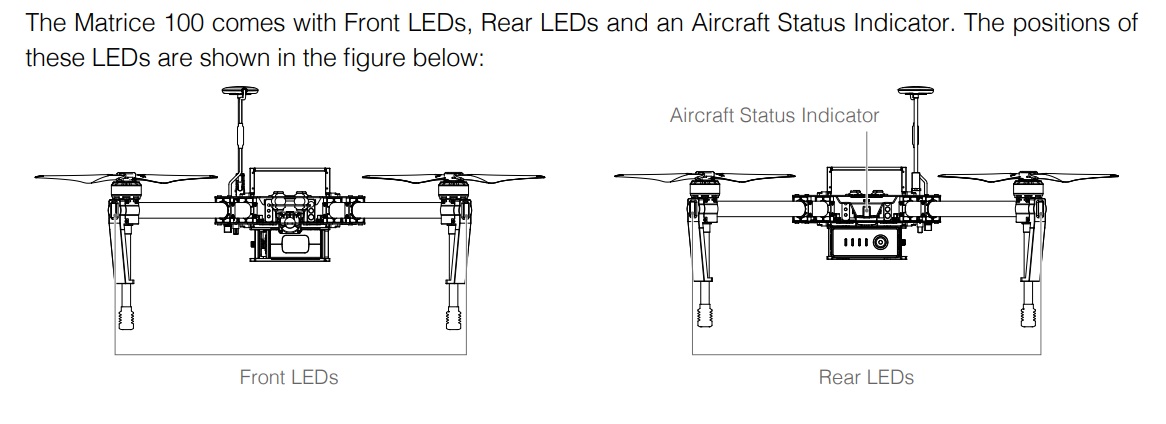
\includegraphics[width=0.8\columnwidth]{figures/op2.png}
\end{center}
\end{figure}  
\begin{figure}[h]
\begin{center}
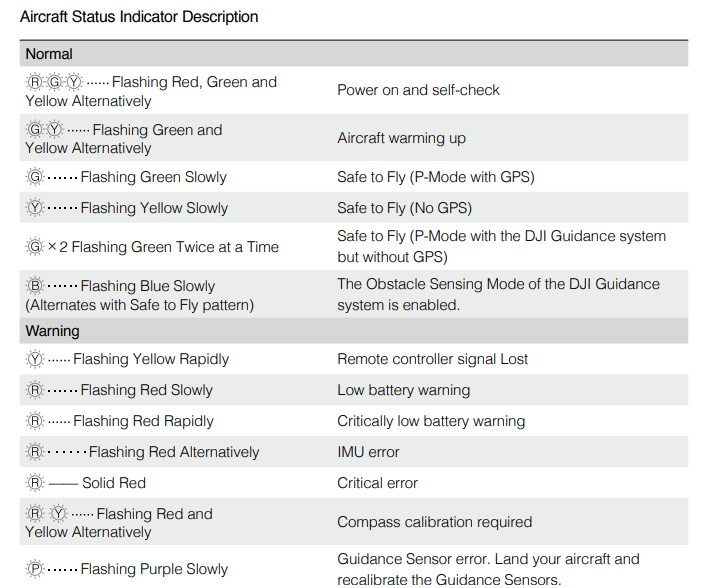
\includegraphics[width=0.6\columnwidth]{figures/op3.png}
\end{center}
\end{figure}  
\item \textbf{DO NOT PROCEED IF WARNING LIGHTS ARE FLASHING}
\item Refer to Aircraft Status Indicator Description chart and resolve issues if applicable. If unresolvable do not operate Matrice until error/warning is resolved. 
\item Ensure extraction device is powered on and operable (when applicable)
\item Prop areas- clear 
\end{enumerate}



\clearpage
\subsubsection{Calibrating Compass Procedure}
\textbf{WARNING:}
\begin{enumerate}
\setlength{\itemsep}{0em}
\setlength{\parskip}{0em}
\item \textbf{DO NOT} Calibrate compass where there is a chance of strong magnetic interference, such as magnetite quarries, parking structures, and underground steel reinforcements
\item \textbf{DO NOT} carry ferromagnetic objects such as keys with you during calibration
\item \textbf{DO NOT} calibrate besides massive metal objects
\item \textbf{DO NOT} calibrate in an indoor space
\end{enumerate}

Proceed once pilot has read through warning section:
\begin{enumerate}
\setlength{\itemsep}{0em}
\setlength{\parskip}{0em}
\item Choose an open space to carry out the procedures
\item Ensure the compass is calibrated. If you did not calibrate the compass as part of your pre-flight preparations, or if you have moved to a new location since the last calibration, tap the System Status bar in the app and select Calibrate, then follow the on-screen instructions to calibrate the aircraft step-by-step
\item Hold the aircraft horizontally, and rotate it 360 degrees along the central axis. The Aircraft Status Indicator will emit a solid green light
\item Hold the aircraft vertically with its nose pointing downwards, and rotate it 360 degrees around its central axis 
\item Recalibrate the compass if the Aircraft Status Indicator becomes solid red
\item If the Aircraft Status Indicator flashes red and yellow alternatively after compass calibration, move your aircraft to a different location to carry out the calibration
\end{enumerate}

\textbf{ALWAYS RECALIBRATE if:}
\begin{enumerate}
\setlength{\itemsep}{0em}
\setlength{\parskip}{0em}
\item The compass data is abnormal, and the Aircraft Status Indicator is flashing red and yellow alternatively 
\item Flying in a new location, or a location that is different from your last flight
\item The mechanical structure of the Matrice 100 is changed, i.e. the mounting position of the GPS module is changed. 
\item Severe drifting occurs in flight, i.e. Matrice 100 has difficulty flying in a straight line. 
\begin{figure}[h]
\begin{center}
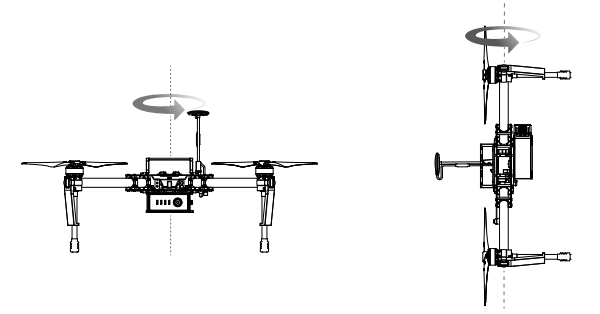
\includegraphics[width=\columnwidth]{figures/op4.png}
\end{center}
\caption{Calibrating compass procedure}
\end{figure}  
\end{enumerate}

  
\clearpage
\subsubsection{Motor Runup}
\begin{enumerate}
\setlength{\itemsep}{0em}
\setlength{\parskip}{0em}
\item Perform Combination Stick Command (CSC) to start/stop the motors. Ensure that you perform the CSC in one continuous motion
\begin{figure}[h]
\begin{center}
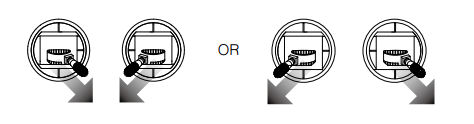
\includegraphics[width=0.7\columnwidth]{figures/op5.png}
\end{center}
\end{figure}  
\item Perform CSC Command. The motors will begin to speed at an idle speed, with the aircraft remaining stationary. 
\item With motors spinning, verify correct rotation
\item At idle, control test (``control surfaces'')- Pitch, roll, yaw
\item Throttle- test to verify response, but do not take off 
\item \textbf{TO STOP MOTORS:} There are two methods:
\begin{enumerate}
\setlength{\itemsep}{0em}
\setlength{\parskip}{0em}
\item Method 1: When the Matrice 100 has landed, push the throttle stick stick down, then perform the CSC command to stop the motors. Release both sticks once the motors have stopped
\item Method 2: When the aircraft has landed, push the throttle down and hold. The motors will stop after a few seconds. 
\end{enumerate}
\begin{figure}[h]
\begin{center}
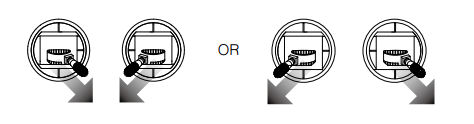
\includegraphics[width=\columnwidth]{figures/op5.png}
\end{center}
\end{figure}   
\item \textbf{DO NOT} perform the CSC command when the aircraft is in mid-air. 
\end{enumerate}

\subsubsection{Before Takeoff}
\begin{enumerate}
\setlength{\itemsep}{0em}
\setlength{\parskip}{0em}
\item Clear- ensure takeoff area is clear
\item Talk- verbally alert other pilots that you are taking off, and state immediate intentions
\end{enumerate}


\clearpage
\subsubsection{Takeoff/Landing Procedures}
\textbf{WARNING:}
\begin{enumerate}
\setlength{\itemsep}{0em}
\setlength{\parskip}{0em}
\item When the Aircraft Status Indicator flashes yellow rapidly during flight, the aircraft has entered Failsafe mode
\item The Aircraft Status Indicator will flash red slowly for a Low Battery Level Warning, and flash red rapidly for a Critically Low Battery Level Warning during flight
\item \textbf{AIRCRAFT WILL LAND AUTOMATICALLY WHEREVER IT IS WHEN REACHING CRITICALLY LOW BATTERY LEVEL WARNING DURING FLIGHT}
\item Recover Aircraft back to home point \textbf{IMMEDIATELY} when Return to Home Status or Low Battery Level Warning is indicated on mobile device or tablet
\item Do not use aircraft in adverse weather conditions including raining, snowing, fog, and wind speeds exceeding (\SI{10}{\meter\per\second})
\item Only fly in open areas. Tall buildings and steel structures may affect accuracy of the compass and the GPS signal
\item Avoid flying near obstacles, crowds, high voltage power lines, trees and bodies of water. 
\item Avoid flying in area with high levels of electromagnetism
\item Aircraft and battery performance is subject to environmental factors such as air density and temperature
\item Matrice 100 cannot operate in P-Mode within the Earth’s polar region

\textbf{IN THE EVENT PILOT HAS LOST GPS SIGNAL AND CAMERA SIGNAL:}
\begin{enumerate}
\setlength{\itemsep}{0em}
\setlength{\parskip}{0em}
\item Alert all personnel that pilot has lost aircraft signal
\item If aircraft is in Field of View and has auto landed at current location, pinpoint and record location for aircraft recovery if recoverable
\item If aircraft is in Field of View and is still operable by remote controller, maneuver aircraft towards the home point \textbf{IMMEDIATELY}
\item \textbf{PROCEED TO RECOVERY PROCEDURE}
\end{enumerate}

Proceed once pilot has read and is aware of above warning section:
\item If applicable, place the aircraft on an open, flat ground with the battery indicator facing you
\item Power on the remote controller and your mobile device, then the Intelligent Flight Battery
\item Launch the DJI GO or RS GO app and enter Camera View
\item Wait until the Aircraft Status Indicator flashes green. This means the Home Point is recorded and is safe to fly. If it flashes yellow, the Home Point has not been recorded and you should not take off
\item Push the throttle stick up slowly to take of or use Auto Takeoff
\item Too land, hover over a level surface and gently pull down on the throttle stick to descend slowly
\item After landing, execute the CSC command or push the throttle stick down for 3 seconds until the motors come to a stop
\item Turn off the Intelligent Flight Battery followed by the remote controller
\end{enumerate}


 
\subsubsection{Recovery Procedure for Boat Operation (if applicable)}
\textbf{WARNING: IN THE EVENT OF CASUALTY DURING RECOVERY PROCEDURE, FOLLOW CASUALTY PROCEDURE IMMEDIATELY. DO NOT PROCEED RECOVERY PROCEDURE}
\begin{enumerate}
\setlength{\itemsep}{0em}
\setlength{\parskip}{0em}
\item Ensure that recovery personnel are strapped with protection gear and standing by at the landing region for recovery. \textbf{DO NOT} proceed if recovery personnel are not ready.
\item Ensure desired landing region is clear of any debris and the person recovering is secured and has given verbal communication to begin recovery
\item Maneuver aircraft so that aircraft is right above landing platform 
\item Adjust gimbal so that camera view is directly on top of recovering personnel and make verbal communication that camera view is centered on landing personnel
\item Announce that you are landing the aircraft to personnel
\item Ensure that personnel are always keeping an eye on the aircraft and must give verbal feedback on aircraft positioning while landing
\item Slowly lower throttle and lower aircraft unless otherwise instructed by recovery personnel
\item Once recovery personnel has secure grip of the aircraft and has given verbal communication that aircraft is secured, \textbf{IMMEDIATELY} perform CSC command to stop motors
\begin{figure}[h]
\begin{center}
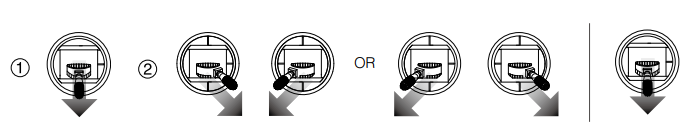
\includegraphics[width=\columnwidth]{figures/op6.png}
\end{center}
\end{figure}  
\item Turn off Flight Battery and remote controller
\end{enumerate}



\clearpage
\subsection{DJI Matrice 100 Post-flight checklist}
\textbf{Note: GPS Mode assumed}

\subsubsection{Walk Around}
\begin{enumerate}
\setlength{\itemsep}{0em}
\setlength{\parskip}{0em}
\item Frame- Check for damage 
\item Screw check- Ensure tightness (frame, standoffs, motors, camera)
\item Wire check- Ensure no damage (fraying, disconnections, etc)
\item Ensure gimbal is not damaged and still operating
\item Ensure extraction device is intact and secured
\item Make sure battery is still working and at operable temperature
\end{enumerate}

\subsubsection{Securing the sample}
\begin{enumerate}
\setlength{\itemsep}{0em}
\setlength{\parskip}{0em}
\item Make sure there is no sharp protruding parts from the extraction device
\item Carefully unlatch sample vessel containing the sample
\item Confirm if sample is the right sample collected and of sufficient size
\end{enumerate}

\subsubsection{In the event of more flights}
\begin{enumerate}
\setlength{\itemsep}{0em}
\setlength{\parskip}{0em}
\item Go through DJI Matrice 100 Pre-flight checklist
\item Ensure extraction device is reset and ready
\item Ensure fully charged battery is used at operable temperature
\end{enumerate}

\subsubsection{Disassembly}
\begin{enumerate}
\setlength{\itemsep}{0em}
\setlength{\parskip}{0em}
\item Ensure the DJI Matrice, controller, and tablet are all turned off
\item Take off propellers and prop guards 
\item Unscrew extraction device from aircraft
\item Unscrew gimbal mount and camera
\item Secure the aircraft components into case
\end{enumerate}